\documentclass[12pt]{article}
\usepackage[utf8]{inputenc}
\usepackage{sbc-template}

\usepackage{graphicx}
\usepackage{graphicx,url}

\usepackage[brazil]{babel}   
%\usepackage[latin1]{inputenc}  
%\usepackage[utf8]{inputenc}
\usepackage[]{xcolor}
% UTF-8 encoding is recommended by ShareLaTex

\usepackage{pdfpages}
\usepackage{listings}
\usepackage{xcolor}

\definecolor{mygreen}{RGB}{28,172,0} % color values Red, Green, Blue
\definecolor{mylilas}{RGB}{170,55,241}

\begin{document}
     
\sloppy

\title{Sistemas de Control Inteligente. \newline Práctica 1: Identificación y control neuronal (II)}

\author{Pablo Acereda García y Laura Pérez Medeiro}


\maketitle


\lstset{language=Matlab,%
    %basicstyle=\color{red},
    backgroundcolor=\color{cyan!10},
    breaklines=true,%
    morekeywords={matlab2tikz},
    keywordstyle=\color{blue},%
    morekeywords=[2]{1}, keywordstyle=[2]{\color{black}},
    identifierstyle=\color{black},%
    stringstyle=\color{mylilas},
    commentstyle=\color{mygreen},%
    showstringspaces=false,%without this there will be a symbol in the places where there is a space
    numbers=left,%
    numberstyle={\tiny \color{black}},% size of the numbers
    numbersep=9pt, % this defines how far the numbers are from the text
    emph=[1]{for,end,break},emphstyle=[1]\color{red}, %some words to emphasise
    %emph=[2]{word1,word2}, emphstyle=[2]{style},    
}

\section{Diseño de un control de posición mediante una red neuronal no recursiva}
\mbox{}
Se pretende diseñar un controlador neuronal capaz de comportarse como un controlador de tipo “caja negra”.
En la práctica se porporciona el bloque de Simulink (controlblackbox.slx), así como el modelo dinámico seguido por el robot, el subsistema de cálculo del error en la posición, los bloques de entrada y salida de información y una serie de restricciones a tener en cuenta.  

\subsection{Implementación del esquema generak de un control de posición dado en el enunciado de la práctica. Además, se deberá configurar los parámetros que participen en la simulación y guardar el esquema con el nombre "PositionControl.slx"}

Para este subapartado del ejercicio es importante tener en cuentaque el sistema debe contar con una condición de parada así como una comprobación para que E\_theta tenga unos valores comprendidos entre %[{-\pi},{\pi}]. 


\begin{figure}[!htb]
    \centering
    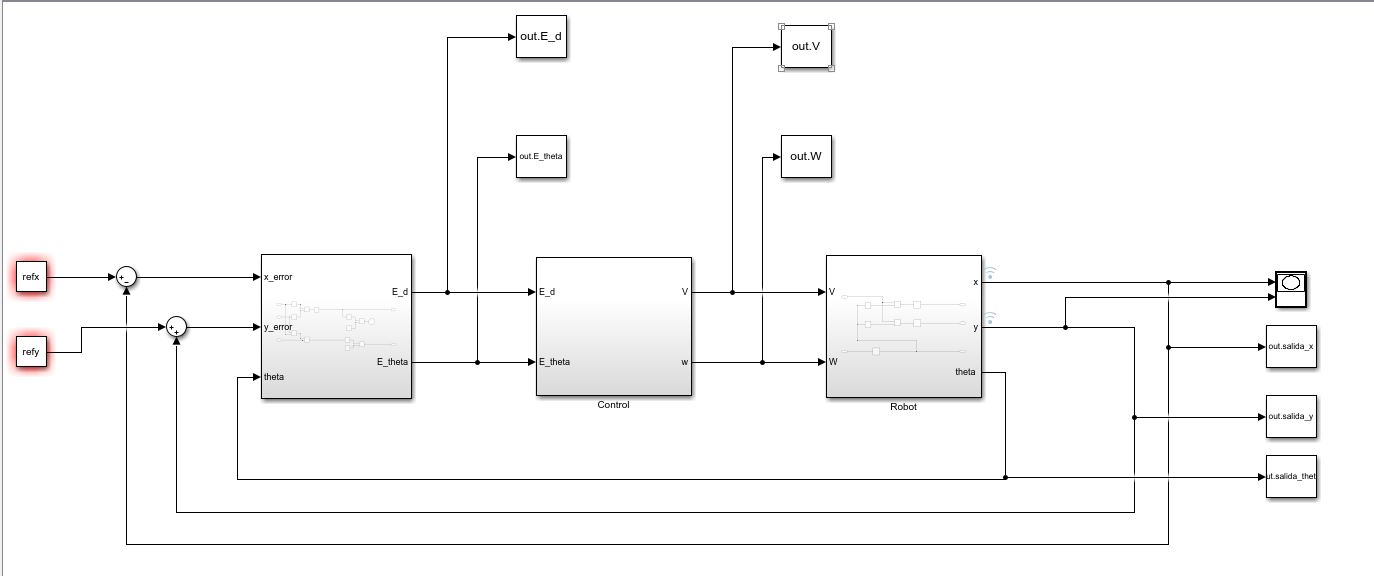
\includegraphics[scale=0.25]{PositionControl.JPG}
\end{figure}


\mbox{}

\subsection{Crear un script con el nombre "RunPositionControl.m, en el cual se pueda simular el diagrama desde el entorno de comonados de Matlab, configurando el punto destino del robot mediante las varaibles refx, refy y Ts.}

\lstinputlisting{codigos/RunPositionControlb.m}

\subsection{Ejecutar el script y comprobar que se generan las variables que contienen las entradas y salidas}

Tras ejecutar el script, podemos ver las variables y sus variables en el workspace situado en la ventana de la derecha.

\subsection{Ejecutar el siguiente código para mostrar la trayectoria del robot mediante el comando plot de Matlab: }

\lstinputlisting{codigos/sectiond.m}

Tras ejecutar ese código obtenemos la siguiente gráfica:
\begin{figure}[!htb]
    \centering
    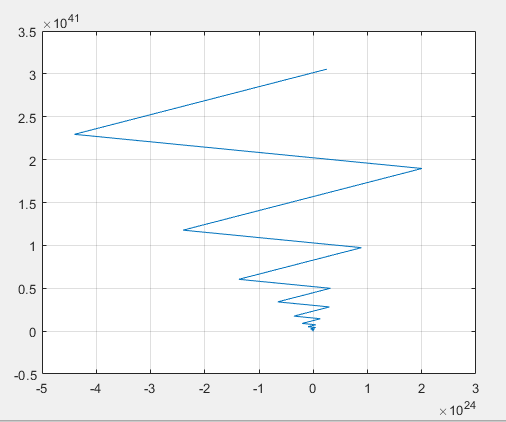
\includegraphics[scale=0.5]{./imagens/TrayectoriaRobot.png}
\end{figure}

\subsection{Realizar N=30 simulaciones del controlador proporcionado valores aleatorios a refx y refy dentro del entorno de 10x10 metros. En cada simulación se deberá guardar el valor de las entradas (E\_d y E\_theta) y salidas (V y W) del bloque controlador. Genere la matriz “inputs” de tamaño 2XN, donde se acumulen los valores de E\_d y E\_theta. Y del mismo la matriz “outputs”, donde se acumulen los valores de V y W. 
 }
\lstinputlisting{codigos/Simulation30Random.m}

\subsection{Diseñar una red neuronal con una capa oculta cuyo comportamiento sea similar al del controlador proporcionado por la práctica. El número de neuronas de la capaoculta deberá elegirse mediante experimentación y justificando su valor}

\section{Generar mediante gensim un bloque con la red neuronal obtenida anteriormente, crear el archivo "PositionControlNet.slx" usando ahora la red neuronal en lugar del controlador y compare los resultados}
\end{document}
